\chapter{Kinematic and Dynamics of Ideal-Fluid Motion}
\section{Kinematic}
\subsection{Streamlines and Vorticity Lines}
\begin{itemize}
\item Streamlines: A curve that is everywhere tangent to the (instantaneous) local velocity vectors.
\item Vorticity lines: A curve that is everywhere tangent to the (instantaneous) local vorticity vectors.
\begin{figure}[H]
\centering
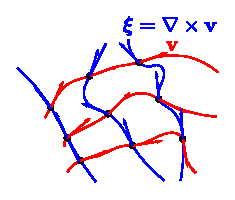
\includegraphics[scale=1.8]{figure/chapter3/3-1-1.eps}
%\caption{\label{fig:blue_rectangle} Rectangle}
\end{figure}
\item Equation of streamline\\
%----------------------
\begin{minipage}{0.4\textwidth}
\begin{equation}
\frac{dx}{u} = \frac{dy}{v} = \frac{dz}{w}
\label{eq: 3-1-1}
\end{equation}
Similarly, for vorticity line
\begin{equation}
\frac{dx}{\xi_x} = \frac{dy}{\xi_y} = \frac{dz}{\xi_z}
\label{eq: 3-1-2}
\end{equation}
\end{minipage} \hfill
\begin{minipage}{0.4\textwidth}
\begin{figure}[H]
\centering
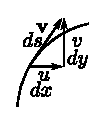
\includegraphics[scale=1.8]{figure/chapter3/3-1-2.eps}
%\caption{\label{fig:blue_rectangle} Rectangle}
\end{figure}
\end{minipage}\\
%----------------------
\item Stream tube and vorticity tube (3D expression)
\begin{figure}[H]
\centering
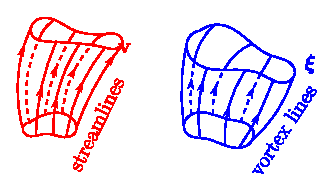
\includegraphics[scale=1.8]{figure/chapter3/3-1-3.eps}
%\caption{\label{fig:blue_rectangle} Rectangle}
\end{figure}
\item Circulation\\
Define circulation\\
%----------------------
\begin{minipage}{0.4\textwidth}
\begin{equation}
\Gamma = \oint_C\mathbf{v}\cdot\mathbf{t}dl
\label{eq: 3-1-3}
\end{equation}
\end{minipage} \hfill
\begin{minipage}{0.4\textwidth}
\begin{figure}[H]
\centering
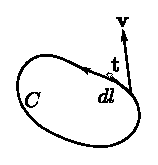
\includegraphics[scale=1.8]{figure/chapter3/3-1-4.eps}
%\caption{\label{fig:blue_rectangle} Rectangle}
\end{figure}
\end{minipage}\\
%----------------------
From Stokes' theorem
\begin{align*}
\Gamma = \oint_C\mathbf{v}\cdot\mathbf{t}dl 
&= \iint_S\mathbf{n}\cdot\left(\nabla\times\mathbf{v}\right) dS \\
&= \iint_S\mathbf{n}\cdot\boldsymbol{\xi}dS
\end{align*}
$\boldsymbol{\xi}=\mathbf{0}$ at all points enclosed in $C\Longrightarrow\Gamma = 0$ around $C$.\\
$\Gamma = 0$ for every loop in the flow field ($\Longrightarrow$circulation-free flow field) \\
$\vc{}{\Longrightarrow}{\xcancel{\Longleftarrow}}\footnotemark \Gamma = 0$ everywhere in the flow field ($\Longrightarrow$irrotational flow field)\footnotetext{can reverted only for simply-connected region}
\item Kinematic of vorticity lines\\
Since $\nabla\cdot\left(\nabla\times\mathbf{v}\right) = 0\Longrightarrow\boxed{\nabla\cdot\boldsymbol{\xi} = 0}$, there can be no source or sink of vorticity, i.e., vorticity line must either forms a closed loop or must terminate on the boundary. (Part of the Helmholtz Theorem). Furthermore, for a closed region $\volume$
\[
{\oiint \hspace{-23.5pt} \int}_{\volume}\nabla\cdot\boldsymbol{\xi}d\volume \vc{=}{\text{div.}}{\text{thm.}} \oiint_S\mathbf{n}\cdot\boldsymbol{\xi}dS = 0
\]
If the closed region is a section of a vorticity tube
%----------------------
\begin{minipage}{0.4\textwidth}
\begin{align*}
&\iint_{S_1}\mathbf{n}\cdot\boldsymbol{\xi}dS + \iint_{S_2}\mathbf{n}\cdot\boldsymbol{\xi}dS = 0 \\
\Longrightarrow
&-\oint_{C_1}\mathbf{v}\cdot\mathbf{t}dl + \oint_{C_2}\mathbf{v}\cdot\mathbf{t}dl = 0\\
\Longrightarrow
&\boxed{\Gamma_{C_1} = \Gamma_{C_2}}\phantom{-} (\abs{\xi_1}S_1=\abs{\xi_2}S_2)
\end{align*}
\end{minipage} \hfill
\begin{minipage}{0.4\textwidth}
\begin{figure}[H]
\centering
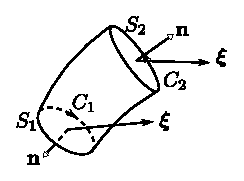
\includegraphics[scale=1.8]{figure/chapter3/3-1-5.eps}
%\caption{\label{fig:blue_rectangle} Rectangle}
\end{figure}
\end{minipage}\\
%----------------------
i.e., the circulation of each cross section of a vorticity tube is a \emph{constant} (Part of the Helmholtz Theorem).
\begin{figure}[H]
\centering
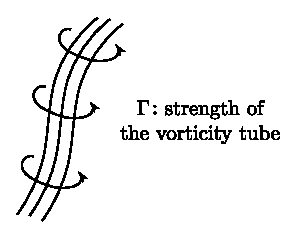
\includegraphics[scale=1.8]{figure/chapter3/3-1-6.eps}
%\caption{\label{fig:blue_rectangle} Rectangle}
\end{figure}
\end{itemize}
\subsection{Stream Function and Potential Function}
\begin{itemize}
\item Potential function\\
A vector field $\mathbf{v}(\mathbf{x},t)$ satisfying $\nabla\times\mathbf{v} = \mathbf{0}$ everywhere is called the \emph{irrotational field}. \\
If $\mathbf{v}$ is velocity field of a flow $\Longrightarrow$ \emph{irrotational field}. \\
Can represent $\mathbf{v}$ by the gradient of a scalar function $\Phi(\mathbf{x},t)$, i.e.
\begin{equation}
\mathbf{v} = \nabla\Phi\text{ (since $\nabla\times\left(\nabla\Phi\right) = \mathbf{0}$)}
\label{eq: 3-1-4}
\end{equation}
where $\Phi$ is scalar (velocity) potential function.
\item Steam function\\
A vector field $\mathbf{v}(\mathbf{x},t)$ satisfying $\nabla\cdot\mathbf{v} = 0$ everywhere is called the \emph{solenoidal field}. \\
If $\mathbf{v}$ is velocity field of a flow $\Longrightarrow$ \emph{solenoidal field}. \\
Can represent $\mathbf{v}$ by the curl of a scalar function $\boldsymbol{\Psi}(\mathbf{x},t)$, i.e.
\begin{equation}
\mathbf{v} = \nabla\times\boldsymbol{\Psi}\text{ (since $\nabla\cdot\left(\nabla\times\boldsymbol{\Psi}\right) = 0$)}
\label{eq: 3-1-5}
\end{equation}
where $\boldsymbol{\Psi}$ is vector potential function. (Note: $\Psi$ is not uniquely determinated by $\mathbf{v}$)
\end{itemize}
Specially for a 2D incompressible flow\\
Since $\mathbf{v} = u(x,y,t)\mathbf{e_x} + v(x,y,t)\mathbf{e_y}$ only, can show that \eqref{eq: 3-1-5} is satisfied with
\[
\boldsymbol{\Psi} = 0\mathbf{e_x} + 0\mathbf{e_y} + \psi(x,y,t)\mathbf{e_z}
\]
where $\psi$ is streamfunction for 2D incompressible flows.
\begin{exercise}
Show that $u\mathbf{e_x} + v\mathbf{e_y} = \nabla\times\boldsymbol{\Psi}$
\end{exercise}
and 
\begin{align*}
u = \frac{\partial\psi}{\partial y}, &&v = -\frac{\partial\psi}{\partial x}
\end{align*}
in polar coordinate, $\psi = \psi(r,\theta,t)$
\begin{align*}
v_r = \frac{1}{r}\frac{\partial\psi}{\partial\theta}, &&v_\theta = - \frac{\partial\psi}{\partial r}
\end{align*}
\begin{exercise}
Show that the vector potential for axisymmetric incompressible flow can be chosen as
\begin{enumerate}[label = \protect\circled{\arabic*}]
\item in cylindrical coordinate ($r,\theta,z$)
\begin{align*}
v_r = v_r(r,z,t), && v_z = v_z(r,z,t), && v_\theta = 0
\end{align*}
\begin{equation}
\boldsymbol{\Psi} = \psi_\theta\mathbf{e_\theta} = \underbrace{\frac{1}{r}\psi(r,z,t)}_{\psi_\theta}\mathbf{e_\theta}
\end{equation}
\[
\nabla\times\boldsymbol{\Psi} = \frac{1}{r}
\begin{vmatrix}
\mathbf{e_r} & r\mathbf{e_\theta} & \mathbf{e_z} \\
\displaystyle\frac{\partial}{\partial r} & \displaystyle\frac{\partial}{\partial\theta} & \displaystyle\frac{\partial}{\partial z} \\
0 & r\psi_\theta & 0
\end{vmatrix}
= v_r\mathbf{e_r} + v_z\mathbf{e_z}
\]
then $\mathbf{v} = \nabla\times\boldsymbol{\Psi}$ 
\begin{align*}
\Longrightarrow
v_r = -\frac{1}{r}\frac{\partial\psi}{\partial z}, && v_z = \frac{1}{r}\frac{\partial\psi}{\partial r}
\end{align*}
where $\psi$ is Stokes' stream function.
\item in spherical coordinate ($r,\theta,\phi$)
\begin{align*}
v_r = v_r(r,\theta,t), && v_\theta = v_\theta(r,\phi,t), && v_\phi = 0
\end{align*}
\begin{equation}
\boldsymbol{\Psi} = \psi_\phi\mathbf{e_\phi} = \underbrace{\frac{1}{r\sin\theta}\psi(r,\theta,t)}_{\psi_\theta}\mathbf{e_\phi}
\end{equation}
\[
\nabla\times\boldsymbol{\Psi} = \frac{1}{r^2\sin\theta}
\begin{vmatrix}
\mathbf{e_r} & r\mathbf{e_\theta} & r\sin\theta\mathbf{e_\phi} \\
\displaystyle\frac{\partial}{\partial r} & \displaystyle\frac{\partial}{\partial\theta} & \displaystyle\frac{\partial}{\partial \phi} \\
0 & 0 & r\sin\theta\psi_\phi\mathbf{e_\phi}
\end{vmatrix}
= v_r\mathbf{e_r} + v_\theta\mathbf{e_\theta}
\]
then $\mathbf{v} = \nabla\times\boldsymbol{\Psi}$ 
\begin{align*}
\Longrightarrow
v_r = \frac{1}{r^2\sin\theta}\frac{\partial\psi}{\partial \theta}, && v_\theta = -\frac{1}{r}\frac{\partial\psi}{\partial r}
\end{align*}
where $\psi$ is Stokes' stream function.
\begin{figure}[H]
\centering
\subfigure[cylindrical coordinate ($r,\theta,z$)]
{
%\label{3-7-Plot of frequency response in amplitude}
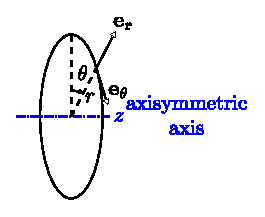
\includegraphics[scale=1.5]{figure/chapter3/3-1-8.eps}
}
\centering
\subfigure[spherical coordinate($r,\theta,\phi$)]
{
%\label{3-7-Plot of frequency response in phase}
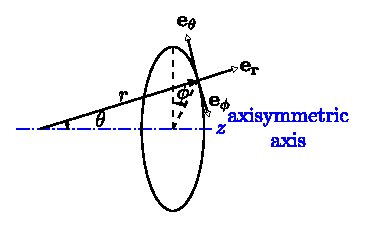
\includegraphics[scale=1.5]{figure/chapter3/3-1-7.eps}
}
%\caption{Plot of frequency response}
\end{figure}
\end{enumerate}
\end{exercise}

\section{Dynamics}
\subsection{Bernoulli equation}
(for inviscid fluid, $\mu = \lambda = 0,\boldsymbol{\tau} = - p\mathbf{I}$ only)\\
Euler equation 
\begin{equation}
\rho\frac{D\mathbf{v}}{Dt} = \rho\mathbf{g} - \nabla p
\label{eq: 3-2-1}
\end{equation}
Now
\[
\frac{D\mathbf{v}}{Dt} = \frac{\partial\mathbf{v}}{\partial t} + \mathbf{v}\cdot\nabla\mathbf{v} = \frac{\partial\mathbf{v}}{\partial t} + \nabla\left(\frac{v^2}{2}\right) - \mathbf{v}\times\boldsymbol{\xi}
\]
\begin{exercise}
Show that vector identity
\[
\mathbf{v}\times\left(\nabla\times\mathbf{v}\right) = \nabla\left(\frac{1}{2}\mathbf{v}\cdot\mathbf{v}\right)- \mathbf{v}\cdot\nabla\mathbf{v} 
\]
\end{exercise}
and $\nabla\times\mathbf{g} = \mathbf{0}$ (conservative force field)\\
$\Longrightarrow\mathbf{g} = -\nabla U$ ($U\colon$ gravitational force)\\
\begin{equation}
\eqref{eq: 3-2-1}\Longrightarrow
\frac{\partial\mathbf{v}}{\partial t} + \nabla\left(\frac{v^2}{2}\right) - \mathbf{v}\times\boldsymbol{\xi} = -\nabla U - \frac{\nabla p}{\rho}
\label{eq: 3-2-2}
\end{equation}
\begin{itemize}
\item  Steady flow along the streamline\\
Let $d\mathbf{s}\parallel$ a special streamline (i.e.$d\mathbf{s}\perp\mathbf{v}$ along streamline)
\[
\begin{aligned}
d\mathbf{s}\cdot\eqref{eq: 3-2-2}
\Longrightarrow &d\mathbf{s}\cdot\nabla\left(\frac{v^2}{2}\right) - \cancelto{0\because\left(\mathbf{v}\times\boldsymbol{\xi}\right)\perp d\mathbf{s}}{d\mathbf{s}\cdot\left(\mathbf{v}\times\mathbf{\xi}\right)}\\ 
&= -d\mathbf{s}\cdot\nabla U - d\mathbf{s}\cdot\frac{\nabla p}{\rho}\\
\Longrightarrow & d\left(\frac{v^2}{2}\right) + \frac{dp}{\rho} + dU = 0
\end{aligned}
\]
integrate (along streamline)
\begin{subequations}
\begin{align}
\Longrightarrow\int\frac{dp}{\rho} + \frac{v^2}{2} + U = \text{ constant (along streamline)}
\label{eq: 3-2-3}
\end{align}
For ideal fluid, $\rho = $ constant
\begin{align}
\eqref{eq: 3-2-3}\Longrightarrow
\frac{p}{\rho} + \frac{v^2}{2} + U = \text{ constant (along streamline)}
\label{eq: 3-2-4}
\end{align}
(Mechanical energy is conserved.)
\end{subequations}
\item Unsteady, \emph{irrotational}, and \emph{barotropic} flow\\
irrotational $\Longrightarrow\boldsymbol{\xi} = \mathbf{0}$ and $\mathbf{v} = \nabla\Phi$\\
barotropic $\Longrightarrow\rho = \rho(p)$ (or $p = p(\rho)$) 
\begin{exercise}
Show that 
\[
\Longrightarrow\frac{\nabla p}{\rho} = \nabla\int\frac{dp}{\rho}
\]
\end{exercise}
\eqref{eq: 3-2-1} reduces to
\[
\nabla\left\{\frac{\partial\Phi}{\partial t} + \frac{v^2}{2} + U + \int\frac{dp}{\rho} = 0\right\}
\]
\begin{equation}
\Longrightarrow\frac{\partial\Phi}{\partial t} + \int\frac{dp}{\rho} + \frac{1}{2}\nabla\Phi\cdot\nabla\Phi + U = f(t)
\label{eq: 3-2-5}
\end{equation}
For steady and incompressible
\[
\eqref{eq: 3-2-5}\Longrightarrow
\boxed{
\frac{p}{\rho} + \frac{1}{2}\nabla\Phi\cdot\nabla\Phi + U = \text{ constant }}
\]
(for ideal fluid + irrotation) everywhere
\end{itemize}
\subsection{Kelvin's Circulation Theorem}
Euler equation
\[
\frac{D\mathbf{v}}{Dt} = -\frac{\nabla p}{\rho} + \frac{\mathbf{f_b}}{\rho}
\]
where $\mathbf{f_b}$ is body force/mass
\begin{figure}[H]
\centering
%\subfigure[cylindrical coordinate ($r,\theta,z$)]
{
%\label{3-7-Plot of frequency response in amplitude}
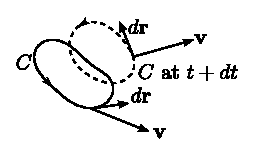
\includegraphics[scale=1.5]{figure/chapter3/3-2-1.eps}
}
\centering
%\subfigure[spherical coordinate($r,\theta,\phi$)]
{
%\label{3-7-Plot of frequency response in phase}
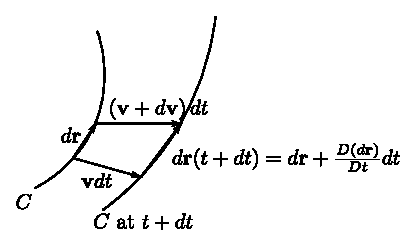
\includegraphics[scale=1.5]{figure/chapter3/3-2-2.eps}
}
%\caption{Plot of frequency response}
\end{figure}
\begin{align*}
&d\mathbf{r} + \left(\mathbf{v} + d\mathbf{v}\right)dt = \mathbf{v}dt + d\mathbf{r} + \frac{D\left(d\mathbf{r}\right)}{Dt}dt \\
\Longrightarrow
&\frac{D\left(d\mathbf{r}\right)}{Dt} = d\mathbf{v}
\end{align*}
or
\[
\frac{D\left(d\mathbf{r}\right)}{Dt} = d\frac{D\mathbf{r}}{Dt} = d\mathbf{v}
\]
Consider around a closed curve curve $C$
\begin{align*}
\Gamma &= \oint_C\mathbf{v}\cdot d\mathbf{r} \\
\frac{D\Gamma}{Dt} &= \frac{D}{Dt}\oint_C\mathbf{v}\cdot d\mathbf{r} \\
&= \oint_C\left[\frac{D\mathbf{v}}{Dt}\cdot d\mathbf{r} + \mathbf{v}\cdot\frac{D\left(d\mathbf{r}\right)}{Dt}\right] \\
&= \oint_C\left[\frac{D\mathbf{v}}{Dt}\cdot d\mathbf{r} + \mathbf{v}\cdot d\mathbf{v}\right]
\end{align*}
Now
\begin{enumerate}[label = \protect\circled{\arabic*}]
\item
\begin{align*}
\oint_C\frac{D\mathbf{v}}{Dt}\cdot d\mathbf{r}
&= \oint_C\left(-\frac{\nabla p}{\rho} + \frac{\mathbf{f_b}}{\rho}\right)\cdot d\mathbf{r} \\
&= \iint_S\mathbf{n}\cdot\mathbf{B} dS
\end{align*}
with
\[
\mathbf{B} = \nabla\times\left[-\frac{\nabla p}{\rho} + \frac{\mathbf{f_b}}{\rho}\right]
\]
\item
\[
\oint_C\mathbf{v}\cdot d\mathbf{v} = \oint_C d\left(\frac{v^2}{2}\right) = 0
\]
as long as no discontinuity in $v^2/2$ existing along the curve $C$
Hence
\begin{equation}
\boxed{\frac{D\Gamma}{Dt} = \iint_S\mathbf{n}\cdot\mathbf{B} dS} \text{ (Bjerknes Theorem)}
\label{eq: 3-2-6}
\end{equation}
i.e., rate of circulation is caused by the rotationality of either surface force $\nabla p /\rho$ or body force $\mathbf{f_b}/\rho$.\\
If the flow is barotropic (i.e. $\rho = \rho (p)$ or $p = p(\rho)$ only)
\[
\frac{\nabla p}{\rho} = \nabla\int\frac{dp}{\rho}
\]
and the body force is conservative, i.e., 
\[
\frac{\mathbf{f_b}}{\rho} = -\nabla U
\]
then
\[
\mathbf{B} = \nabla\times\left[-\nabla\int\frac{dp}{\rho} - \nabla U\right] = \mathbf{0}
\]
\begin{equation}
\boxed{
\frac{D\Gamma}{Dt} = 0
}\text{ (Kelvin's Theorem)}
\label{eq: 3-2-7}
\end{equation}
i.e., circulation around any closed material curve is \emph{conserved} in an \emph{inviscid}, \emph{barotropic} (or $\rho =$ constant), and \emph{conservative body force field}. 
%\input{test.tex}
\end{enumerate}

\begin{discussion}\mbox{}\\
\begin{enumerate}[label = \protect\circled{\arabic*}]
\item The flow does not have to be irrotational ($\boldsymbol{\xi}=\mathbf{0}$)
\item Kelvin's theorem implies that all motions started from rest (i.e., $\Gamma = 0$ for every loop initially) must be circulation free (i.e. irrotational) at any subsequent instant.
\item Eq .\eqref{eq: 3-2-7} also applies to

%
\begin{tikzpicture} 
\coordinate (C1) at (1.2,0);
\node[below right] at (C1){$C$};
\coordinate (C2) at (2.2,0);
\node[below right] at (C2){$C'$};
\coordinate (C3) at (3.2,0);
\node[below right] at (C3){$C''$};
\coordinate (C4) at (4.2,0);
\node[right] at (C4){$\displaystyle\frac{D\Gamma}{Dt} = 0$};
\draw[->] (-3,1) -- (-2,1);
\draw[->] (-3,0) -- (-2,0);
\draw[->] (-3,-1) -- (-2,-1);
\filldraw[color=blue!60, fill=blue!10](0,0) circle (1);
\draw[color=blue!60 ,pattern=hatch, pattern color=blue!60, hatch size=10pt, hatch angle=0](0,0) circle (1);

% \draw (2.5,0) ellipse (1.5 and 0.5);
\draw [-{Latex[length=2mm]}, rotate=0] (C1) arc [start angle=-360, end angle=0, x radius=1.2cm, y radius=1.2cm];
\draw [-{Latex[length=2mm]}, rotate=0] (C2) arc [start angle=-360, end angle=0, x radius=1.8cm, y radius=1.4cm];
\draw [-{Latex[length=2mm]}, rotate=0] (C3) arc [start angle=-360, end angle=0, x radius=2.4cm, y radius=1.6cm];
\end{tikzpicture}

\vspace{5em}

\begin{tikzpicture}[scale=6,transform canvas]
\newcommand{\la}{0.5}
\newcommand{\lb}{-0.1}
\begin{scope}[rotate=-5]
	\filldraw[color=blue!60, fill=blue!10, line width=0.04mm] 
(1.0000000,0.0005993) -- 
(0.9900000,0.0029690) --
(0.9800000,0.0053335) -- 
(0.9700000,0.0076868) -- 
(0.9600000,0.0100232) -- 
(0.9400000,0.0146239) -- 
(0.9200000,0.0191156) -- 
(0.9000000,0.0235025) -- 
(0.8800000,0.0277891) -- 
(0.8600000,0.0319740) -- 
(0.8400000,0.0360536) -- 
(0.8200000,0.0400245) -- 
(0.8000000,0.0438836) -- 
(0.7800000,0.0476281) -- 
(0.7600000,0.0512565) -- 
(0.7400000,0.0547675) -- 
(0.7200000,0.0581599) -- 
(0.7000000,0.0614329) -- 
(0.6800000,0.0645843) -- 
(0.6600000,0.0676046) -- 
(0.6400000,0.0704822) -- 
(0.6200000,0.0732055) -- 
(0.6000000,0.0757633) -- 
(0.5800000,0.0781451) -- 
(0.5600000,0.0803480) -- 
(0.5400000,0.0823712) -- 
(0.5200000,0.0842145) -- 
(0.5000000,0.0858772) -- 
(0.4800000,0.0873572) -- 
(0.4600000,0.0886427) -- 
(0.4400000,0.0897175) -- 
(0.4200000,0.0905657) -- 
(0.4000000,0.0911712) -- 
(0.3800000,0.0915212) -- 
(0.3600000,0.0916266) -- 
(0.3400000,0.0915079) -- 
(0.3200000,0.0911857) -- 
(0.3000000,0.0906804) -- 
(0.2800000,0.0900016) -- 
(0.2600000,0.0890840) -- 
(0.2400000,0.0878308) -- 
(0.2200000,0.0861433) -- 
(0.2000000,0.0839202) -- 
(0.1800000,0.0810687) -- 
(0.1600000,0.0775707) -- 
(0.1400000,0.0734360) -- 
(0.1200000,0.0686204) -- 
(0.1000000,0.0629981) -- 
(0.0800000,0.0564308) -- 
(0.0600000,0.0487571) -- 
(0.0500000,0.0442753) -- 
(0.0400000,0.0391283) -- 
(0.0300000,0.0330215) -- 
(0.0200000,0.0253735) -- 
(0.0120000,0.0178581) -- 
(0.0080000,0.0137350) -- 
(0.0040000,0.0089238) -- 
(0.0020000,0.0058025) -- 
(0.0010000,0.0037271) -- 
(0.0005000,0.0023390) -- 
(0.0000000,0.0000000) coordinate (y) -- 
(0.0005000,-.0046700) -- 
(0.0010000,-.0059418) -- 
(0.0020000,-.0078113) -- 
(0.0040000,-.0105126) -- 
(0.0080000,-.0142862) -- 
(0.0120000,-.0169733) -- 
(0.0200000,-.0202723) -- 
(0.0300000,-.0226056) -- 
(0.0400000,-.0245211) -- 
(0.0500000,-.0260452) -- 
(0.0600000,-.0271277) -- 
(0.0800000,-.0284595) -- 
(0.1000000,-.0293786) -- 
(0.1200000,-.0299633) -- 
(0.1400000,-.0302404) -- 
(0.1600000,-.0302546) -- 
(0.1800000,-.0300490) -- 
(0.2000000,-.0296656) -- 
(0.2200000,-.0291445) -- 
(0.2400000,-.0285181) -- 
(0.2600000,-.0278164) -- 
(0.2800000,-.0270696) -- 
(0.3000000,-.0263079) -- 
(0.3200000,-.0255565) -- 
(0.3400000,-.0248176) -- 
(0.3600000,-.0240870) -- 
(0.3800000,-.0233606) -- 
(0.4000000,-.0226341) -- 
(0.4200000,-.0219042) -- 
(0.4400000,-.0211708) -- 
(0.4600000,-.0204353) -- 
(0.4800000,-.0196986) -- 
(0.5000000,-.0189619) -- 
(0.5200000,-.0182262) -- 
(0.5400000,-.0174914) -- 
(0.5600000,-.0167572) -- 
(0.5800000,-.0160232) -- 
(0.6000000,-.0152893) -- 
(0.6200000,-.0145551) -- 
(0.6400000,-.0138207) -- 
(0.6600000,-.0130862) -- 
(0.6800000,-.0123515) -- 
(0.7000000,-.0116169) -- 
(0.7200000,-.0108823) -- 
(0.7400000,-.0101478) -- 
(0.7600000,-.0094133) -- 
(0.7800000,-.0086788) -- 
(0.8000000,-.0079443) -- 
(0.8200000,-.0072098) -- 
(0.8400000,-.0064753) -- 
(0.8600000,-.0057408) -- 
(0.8800000,-.0050063) -- 
(0.9000000,-.0042718) -- 
(0.9200000,-.0035373) -- 
(0.9400000,-.0028028) -- 
(0.9600000,-.0020683) -- 
(0.9700000,-.0017011) -- 
(0.9800000,-.0013339) -- 
(0.9900000,-.0009666) -- 
(1.0000000,-.0005993) coordinate (x);
%
\draw[color=blue!60 ,pattern=hatch, pattern color=blue!60, hatch size=10pt, hatch angle=0]
(1.0000000,0.0005993) -- 
(0.9900000,0.0029690) -- 
(0.9800000,0.0053335) -- 
(0.9700000,0.0076868) -- 
(0.9600000,0.0100232) -- 
(0.9400000,0.0146239) -- 
(0.9200000,0.0191156) -- 
(0.9000000,0.0235025) -- 
(0.8800000,0.0277891) -- 
(0.8600000,0.0319740) -- 
(0.8400000,0.0360536) -- 
(0.8200000,0.0400245) -- 
(0.8000000,0.0438836) -- 
(0.7800000,0.0476281) -- 
(0.7600000,0.0512565) -- 
(0.7400000,0.0547675) -- 
(0.7200000,0.0581599) -- 
(0.7000000,0.0614329) -- 
(0.6800000,0.0645843) -- 
(0.6600000,0.0676046) -- 
(0.6400000,0.0704822) -- 
(0.6200000,0.0732055) -- 
(0.6000000,0.0757633) -- 
(0.5800000,0.0781451) -- 
(0.5600000,0.0803480) -- 
(0.5400000,0.0823712) -- 
(0.5200000,0.0842145) -- 
(0.5000000,0.0858772) -- 
(0.4800000,0.0873572) -- 
(0.4600000,0.0886427) -- 
(0.4400000,0.0897175) -- 
(0.4200000,0.0905657) -- 
(0.4000000,0.0911712) -- 
(0.3800000,0.0915212) -- 
(0.3600000,0.0916266) -- 
(0.3400000,0.0915079) -- 
(0.3200000,0.0911857) -- 
(0.3000000,0.0906804) -- 
(0.2800000,0.0900016) -- 
(0.2600000,0.0890840) -- 
(0.2400000,0.0878308) -- 
(0.2200000,0.0861433) -- 
(0.2000000,0.0839202) -- 
(0.1800000,0.0810687) -- 
(0.1600000,0.0775707) -- 
(0.1400000,0.0734360) -- 
(0.1200000,0.0686204) -- 
(0.1000000,0.0629981) -- 
(0.0800000,0.0564308) -- 
(0.0600000,0.0487571) -- 
(0.0500000,0.0442753) -- 
(0.0400000,0.0391283) -- 
(0.0300000,0.0330215) -- 
(0.0200000,0.0253735) -- 
(0.0120000,0.0178581) -- 
(0.0080000,0.0137350) -- 
(0.0040000,0.0089238) -- 
(0.0020000,0.0058025) -- 
(0.0010000,0.0037271) -- 
(0.0005000,0.0023390) -- 
(0.0000000,0.0000000) -- 
(0.0005000,-.0046700) -- 
(0.0010000,-.0059418) -- 
(0.0020000,-.0078113) -- 
(0.0040000,-.0105126) -- 
(0.0080000,-.0142862) -- 
(0.0120000,-.0169733) -- 
(0.0200000,-.0202723) -- 
(0.0300000,-.0226056) -- 
(0.0400000,-.0245211) -- 
(0.0500000,-.0260452) -- 
(0.0600000,-.0271277) -- 
(0.0800000,-.0284595) -- 
(0.1000000,-.0293786) -- 
(0.1200000,-.0299633) -- 
(0.1400000,-.0302404) -- 
(0.1600000,-.0302546) -- 
(0.1800000,-.0300490) -- 
(0.2000000,-.0296656) -- 
(0.2200000,-.0291445) -- 
(0.2400000,-.0285181) -- 
(0.2600000,-.0278164) -- 
(0.2800000,-.0270696) -- 
(0.3000000,-.0263079) -- 
(0.3200000,-.0255565) -- 
(0.3400000,-.0248176) -- 
(0.3600000,-.0240870) -- 
(0.3800000,-.0233606) -- 
(0.4000000,-.0226341) -- 
(0.4200000,-.0219042) -- 
(0.4400000,-.0211708) -- 
(0.4600000,-.0204353) -- 
(0.4800000,-.0196986) -- 
(0.5000000,-.0189619) -- 
(0.5200000,-.0182262) -- 
(0.5400000,-.0174914) -- 
(0.5600000,-.0167572) -- 
(0.5800000,-.0160232) -- 
(0.6000000,-.0152893) -- 
(0.6200000,-.0145551) -- 
(0.6400000,-.0138207) -- 
(0.6600000,-.0130862) -- 
(0.6800000,-.0123515) -- 
(0.7000000,-.0116169) -- 
(0.7200000,-.0108823) -- 
(0.7400000,-.0101478) -- 
(0.7600000,-.0094133) -- 
(0.7800000,-.0086788) -- 
(0.8000000,-.0079443) -- 
(0.8200000,-.0072098) -- 
(0.8400000,-.0064753) -- 
(0.8600000,-.0057408) -- 
(0.8800000,-.0050063) -- 
(0.9000000,-.0042718) -- 
(0.9200000,-.0035373) -- 
(0.9400000,-.0028028) -- 
(0.9600000,-.0020683) -- 
(0.9700000,-.0017011) -- 
(0.9800000,-.0013339) -- 
(0.9900000,-.0009666) -- 
(1.0000000,-.0005993);;
\end{scope}
\coordinate (z) at (y |- x);
\coordinate (vtip) at ($(x) + (\la,\lb)$);
\node[below] at ($(vtip) + (0.02,0)$){vortex sheet};

\draw[-] (x.east) .. controls +(down:0mm) and +(left:1mm) .. (vtip.west);
\coordinate (vtip middle) at ($(x)!0.25!(vtip)$);
\coordinate (vtip middle top) at ($(vtip middle) + (0,0.2)$);
\coordinate (vtip middle bottom) at ($(vtip middle) + (0,-0.2)$);
\draw[-] (vtip middle) -- (vtip middle top);
\draw[-] (vtip middle) -- (vtip middle bottom); 

\foreach \v in {0.2,0.4,0.6,0.8}{
	\draw[->]  ($(vtip middle)!\v!(vtip middle top)$) -- ($(vtip middle)!\v!(vtip middle top) + (0.2,0)$);    
    }
%
\foreach \v in {0.2,0.4,0.6,0.8}{
	\draw[->]  ($(vtip middle)!\v!(vtip middle bottom)$) -- ($(vtip middle)!\v!(vtip middle bottom) + (0.1,0)$);    
    }
\draw [-{Latex[length=2mm]}, rotate=0] ($(vtip) + (-0.48, 0.5)$) arc [start angle=-300, end angle=60, x radius=0.7cm, y radius=0.45cm];
\node[above right] at ($(vtip) + (-0.5, 0.5)$){$\displaystyle C'\rightarrow\frac{D\Gamma}{Dt}\neq 0$};
\draw [-{Latex[length=2mm]}, rotate=0] ($(vtip) + (0.24,-0.05)$) arc [start angle=-380, end angle=-20, x radius=1.0cm, y radius=0.6cm];
\node[below right] at ($(vtip) + (0.2,-0.05)$){$\displaystyle C\rightarrow\frac{D\Gamma}{Dt}= 0$};
\end{tikzpicture}

\vspace{5em}

\item \mbox{}\\ 
\begin{enumerate}[label = (\alph*)]
\item \label{ch3-2-dis-a} Helmholtz theorem: $\Gamma =$constant around the cross-section of a vorticity tube
\item \label{ch3-2-dis-b} Kelvin's theorem: $\Gamma =$constant around a material closed curve 
\item \label{ch3-2-dis-c} Can show that Kelvin's theorem $\Longrightarrow$ vorticity line is a material 
\end{enumerate}
i.e., once a vorticity line (tube), always a vorticity line (tube).\\
Hence \ref{ch3-2-dis-a} + \ref{ch3-2-dis-b} + \ref{ch3-2-dis-c} $\Longrightarrow$ circulation $\Gamma$ around a vorticity tube is preserved along its motion (in an inviscid, barotropic, and conservative-body force field)
\begin{figure}[H]
\centering
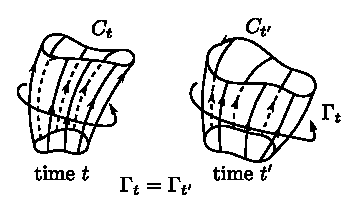
\includegraphics[scale=1.8]{figure/chapter3/3-2-5.eps}
%\caption{\label{fig:blue_rectangle} Rectangle}
\end{figure}
\item Summary of the Helmholtz Vortex Theorem
\begin{enumerate}[label = (\alph*)]
\item $\nabla\cdot\boldsymbol{\xi} = 0\Longrightarrow$ Vorticity line either forms a closed loop or terminate at boundary
\item \label{ch3-2-dis-4-b}
\[
\iint_{S_1}\mathbf{n}\cdot\boldsymbol{\xi}dS = -\iint_{S_2}\mathbf{n}\cdot\boldsymbol{\xi}dS\Longrightarrow\Gamma_{C_1}=\Gamma_{C_2}
\]
\begin{figure}[H]
\centering
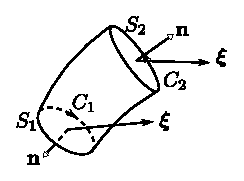
\includegraphics[scale=1.8]{figure/chapter3/3-2-6.eps}
%\caption{\label{fig:blue_rectangle} Rectangle}
\end{figure}
\item \label{ch3-2-dis-4-c} Vorticity line is a material line (in an inviscid, barotropic, and conservative-body force field)
\item \label{ch3-2-dis-4-d} $\displaystyle\frac{D\Gamma}{Dt}=0$ along any material closed curve, e.g. vortex ring\\
\begin{tikzpicture}
\begin{scope}[rotate=-30]
    \draw [-{Latex[length=2mm]}, rotate=0] ($(0, 0) + (2, 1.2)$) arc [start angle=60, end angle=220, x radius=0.9cm, y radius=0.8cm];
    \draw [-{Latex[length=2mm]}, rotate=0] ($(0, 0) + (-2, 1.2)$) arc [start angle=120, end angle=-40, x radius=0.9cm, y radius=0.8cm];
    \draw [-{Latex[length=2mm]}, rotate=0] ($(0, 0) + (-0.2, -1.7)$) arc [start angle=270, end angle=450, x radius=0.9cm, y radius=0.8cm];
    \draw (0,0) ellipse (3 and 1.5);
    \clip (0,-1.8) ellipse (3 and 2.5);
    \draw (0,2.2) ellipse (3 and 2.5);
    \clip (0,2.2) ellipse (3 and 2.5);
    \draw (0,-2.2) ellipse (3 and 2.5);
\end{scope}
\end{tikzpicture}
\item From \ref{ch3-2-dis-4-b} + \ref{ch3-2-dis-4-c} + \ref{ch3-2-dis-4-d} $\Longrightarrow$ circulation around a vorticity tube is preserved along its motion (in an inviscid, barotropic, and conservative-body force field)
\end{enumerate}
\end{enumerate}
\end{discussion}
\subsection{Vorticity Equation}
Euler Equation
\[
\frac{\partial\mathbf{v}}{\partial t} + \mathbf{v}\cdot\nabla\mathbf{v} = \frac{1}{\rho}\mathbf{g} - \frac{\nabla p}{\rho}
\]
\begin{equation}
\Longrightarrow
\frac{\partial\mathbf{v}}{\partial t} + \nabla\left(\frac{v^2}{2}\right) - \mathbf{v}\times\boldsymbol{\xi} = -\nabla U - \frac{\nabla p}{\rho}
\tag{$\ast$}
\label{eq: ch3-2-3-*}
\end{equation}
\begin{equation}
\nabla\times\eqref{eq: ch3-2-3-*}\Longrightarrow\frac{\partial\boldsymbol{\xi}}{\partial t} + 0 - \nabla\times\left(\mathbf{v}\times\boldsymbol{\xi}\right) = 0 - \nabla\times\left(\frac{\nabla p}{\rho}\right)
\tag{$\ast\ast$}
\label{eq: ch3-2-3-**}
\end{equation}
From vector identity
\[
\nabla\times\left(\mathbf{v}\times\boldsymbol{\xi}\right) = \mathbf{v}\cancelto{0}{\left(\nabla\cdot\boldsymbol{\xi}\right)} - \underbrace{\boldsymbol{\xi}\left(\nabla\cdot\mathbf{v}\right)}_{\nabla\cdot\mathbf{v}=-\frac{1}{\rho}\frac{D\rho}{Dt}} + \left(\boldsymbol{\xi}\cdot\nabla\right)\mathbf{v} - \left(\mathbf{v}\cdot\nabla\right)\boldsymbol{\xi}
\]
also
\begin{exercise}
\begin{align*}
\nabla\times\left(\frac{\nabla p}{\rho}\right) 
&= \frac{1}{\rho}\cancelto{0}{\nabla\times\nabla p} + \left(\nabla\frac{1}{\rho}\right)\times\nabla p \\
&= -\frac{1}{\rho^2}\nabla \rho\times\nabla p
\end{align*}
\end{exercise}
\begin{exercise}
\begin{equation}
\eqref{eq: ch3-2-3-**}\Longrightarrow
\frac{D}{Dt}\left(\frac{\boldsymbol{\xi}}{\rho}\right) = \frac{\boldsymbol{\xi}}{\rho}\cdot\nabla\mathbf{v} + \frac{1}{\rho^2}\nabla\rho\times\nabla p
\label{eq: 3-2-8}
\end{equation}
\end{exercise}
For barotropic flow ($\rho=\rho (p)$ or $p=p(\rho)$)
\[
p = p(\rho)\Longrightarrow\nabla p = \frac{dp}{d\rho}\nabla\rho\Longrightarrow\nabla p\parallel\nabla\rho\Longrightarrow\nabla\rho\times\nabla p = 0
\]
\begin{equation}
\eqref{eq: 3-2-8}\Longrightarrow\frac{D}{Dt}\left(\frac{\boldsymbol{\xi}}{\rho}\right) = \frac{\boldsymbol{\xi}}{\rho}\cdot\nabla\mathbf{v}
\label{eq: 3-2-9}
\end{equation}
(in an inviscid, barotropic, and conservative-body force field)\\
For ideal fluid ($\rho=$constant)
\begin{equation}
\eqref{eq: 3-2-8}\Longrightarrow
\boxed{
\frac{D\boldsymbol{\xi}}{Dt} = \boldsymbol{\xi}\cdot\nabla\mathbf{v}
}
\label{eq: 3-2-10}
\end{equation}
\begin{itemize}
\item In an inviscid, barotropic (or $\rho=$ constant) and conservative body-force field, a vorticity line is a material line.
\begin{equation}
\Longrightarrow
\frac{D\left(d\mathbf{r}\right)}{Dt} = d\mathbf{v} = d\mathbf{r}\cdot\nabla\mathbf{v}
\label{eq: 3-2-11}
\end{equation}
\begin{figure}[H]
\centering
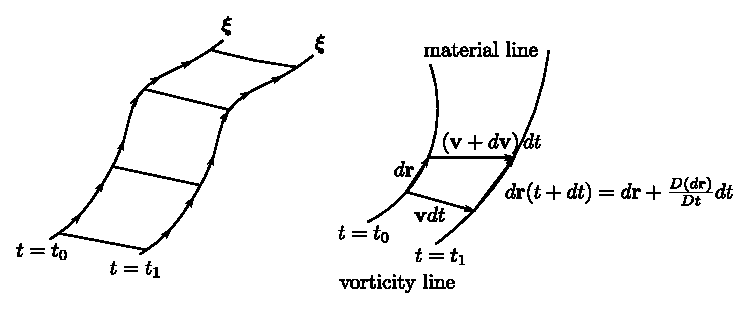
\includegraphics[scale=1.5]{figure/chapter3/3-2-7.eps}
%\caption{\label{fig:blue_rectangle} Rectangle}
\end{figure}
Now let $d\mathbf{r}$ be a segment of a vorticity line at $t=t_0$, i.e.
\[
\boldsymbol{\xi}\times d\mathbf{r} = \mathbf{0}\text{ (or $\boldsymbol{\xi}=\lambda d\mathbf{r}$) at } t=t_0
\]
\begin{align*}
\left[\frac{D\left(\boldsymbol{\xi}\times d\mathbf{r}\right)}{Dt}\right]_{t_0}
&= \left(\frac{D\boldsymbol{\xi}}{Dt}\times d\mathbf{r}\right)_{t_0} + \left(\boldsymbol{\xi}\times\frac{D\left(d\mathbf{r}\right)}{Dt}\right)_{t_0} \\
&= \left[\left(\boldsymbol{\xi}\cdot\nabla\mathbf{v}\right)\times d\mathbf{r}\right]_{t_0} + \left[\boldsymbol{\xi}\times d\mathbf{v}\right]_{t_0} \\
&= \left[\left(\lambda d\mathbf{r}\cdot\nabla\mathbf{v}\right)\times d\mathbf{r}\right]_{t_0} + \left[\lambda d\mathbf{r}\times d\mathbf{v}\right]_{t_0} \\
&= \left[\left(\lambda d\mathbf{v}\right)\times d\mathbf{r}\right]_{t_0} + \left[\lambda d\mathbf{r}\times d\mathbf{v}\right]_{t_0} = \mathbf{0}
\end{align*}
\[
\Longrightarrow \left(\boldsymbol{\xi}\times d\mathbf{r}\right)_{t+dt} = \left(\boldsymbol{\xi}\times d\mathbf{r}\right)_{t_0}
\]
\item The term $\boldsymbol{\xi}\cdot\nabla\mathbf{v}$ in vorticity equation
%----------------------
\begin{minipage}{0.4\textwidth}
Let $\boldsymbol{\xi}=\lambda d\mathbf{r}$\\
$\displaystyle\lambda(\mathbf{x},t) = \frac{\abs{\boldsymbol{\xi}}}{\abs{d\mathbf{r}}}$ vorticity/unit length\\
$\lambda\colon$ vorticity density
\end{minipage} \hfill
\begin{minipage}{0.4\textwidth}
\begin{figure}[H]
\centering
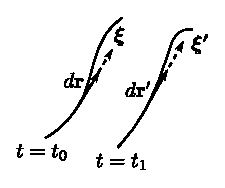
\includegraphics[scale=1.8]{figure/chapter3/3-2-8.eps}
%\caption{\label{fig:blue_rectangle} Rectangle}
\end{figure}
\end{minipage}\\
%----------------------
then 
\[
\frac{D\boldsymbol{\xi}}{Dt} = \boldsymbol{\xi}\cdot\nabla\mathbf{v}\Longrightarrow\frac{D\left(\lambda d\mathbf{r}\right)}{Dt} = \lambda d\mathbf{r}\cdot\nabla\mathbf{v}
\]
\[
\Longrightarrow\frac{D\lambda}{Dt}d\mathbf{r} + \lambda\underbrace{\frac{D\left(d\mathbf{r}\right)}{Dt}}_{d\mathbf{v}=d\mathbf{r}\cdot\nabla\mathbf{v}} = \lambda d\mathbf{r}\cdot\nabla\mathbf{v}
\]
\[
\Longrightarrow\boxed{\frac{D\lambda}{Dt} = 0}
\]
i.e., $\lambda$ is conserved when following fluid motion
\begin{figure}[H]
\centering
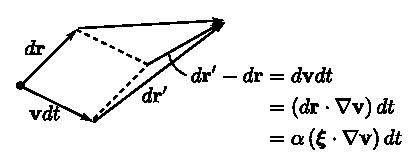
\includegraphics[scale=1.8]{figure/chapter3/3-2-9.eps}
%\caption{\label{fig:blue_rectangle} Rectangle}
\end{figure}
i.e., \emph{stretching} and \emph{turning} of the vorticity line in $dt$ is caused by the \emph{deformation rate field $\nabla\mathbf{v}$}.
\end{itemize}
\begin{note}\mbox{}\\
\begin{enumerate}[label = \protect\circled{\arabic*}]
\item The term $\boldsymbol{\xi}\cdot\nabla\mathbf{v}$ has important consequence in turbulent flow 
\begin{figure}[H]
\centering
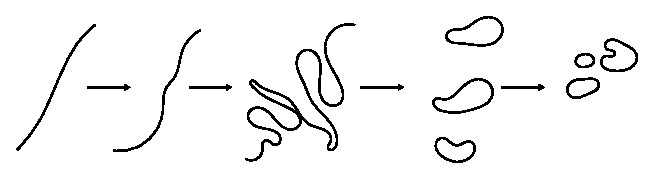
\includegraphics[scale=1.5]{figure/chapter3/3-2-10.eps}
%\caption{\label{fig:blue_rectangle} Rectangle}
\end{figure}
\item vorticity stretching effect
\begin{figure}[H]
\centering
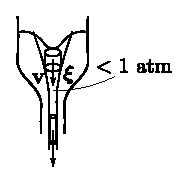
\includegraphics[scale=1.8]{figure/chapter3/3-2-11.eps}
%\caption{\label{fig:blue_rectangle} Rectangle}
\end{figure}
\end{enumerate}
\end{note}
